\bookchapter{Bab 60: Menyiapkan Lingkungan Pengembangan — Xcode dan Proyek Pertama}

\chapterintro{Ingin bekerja bagus, tajamkan dulu alatnya. Di bab ini kita menata “dapur”: memasang Xcode, menjalankan Simulator sampai jalan, membuat proyek iOS pertama dalam hidupmu, lalu membongkar struktur proyeknya sampai jelas. Setelah lingkungan siap, kamu akan pertama kali melihat kode tulisanmu menjadi tombol yang bisa ditekan — momen ini bagi banyak orang diingat seumur hidup.}

\booksection{Siapkan sebuah Mac}

Syaratnya dulu: pengembangan iOS harus dilakukan di macOS. Kalau belum punya Mac, pilihannya tiga: beli satu (Mac mini atau MacBook Air bekas pun cukup), sewa Mac cloud untuk jangka pendek, atau baca dulu Bagian 8 “Praktik Pengembangan Android” (bisa dikerjakan di Windows).

\begin{center}
\begin{tabularx}{\linewidth}{|X|X|X|}
\hline
\textbf{Butir spesifikasi} & \textbf{Kebutuhan minimum} & \textbf{Batas nyaman (direkomendasikan)} \tabularnewline
\hline
Chip & Apple Silicon (M1 ke atas) & M2 atau lebih baru \tabularnewline
Memori & 8GB & 16GB \tabularnewline
Disk & Sediakan 40GB+ (badan Xcode sendiri gemuk) & Mulai dari 256GB \tabularnewline
Sistem & macOS terbaru & Biarkan pembaruan otomatis menyala \tabularnewline
\hline
\end{tabularx}
\end{center}

\begin{center}\small\color{gray}Referensi konfigurasi Mac untuk pengembangan (Agustus 2026)\end{center}

\begin{tcbinfo}{Tips: Tanpa Mac pun bisa belajar bahasanya dulu}
Swift Playgrounds yang gratis di iPad bisa dipakai mempelajari dasar bahasa Swift (tanpa Mac); bahkan bisa dipasang di iPhone. Mainkan dulu materi bahasa Bab 61 di Playgrounds sampai cair, begitu Mac tiba langsung melesat. “Mengasah parang tak menunda menebang kayu” — maksudnya persis itu.

\end{tcbinfo}

\booksection{Memasang Xcode}

Xcode adalah lingkungan pengembangan terintegrasi resmi Apple, gratis. Terpasang dalam tiga langkah:

\begin{enumerate}
  \item Di Mac buka App Store, cari "Xcode", tekan pasang — perhatikan ukurannya beberapa GB, pilih waktu dengan jaringan bagus;
  \item Setelah terpasang, saat pertama dijalankan: setujui perjanjian, tunggu komponen selesai terpasang (otomatis);
  \item Menu Xcode Settings Locations, pastikan Command Line Tools sudah terpilih — alat baris perintah adalah prasyarat banyak skrip dan alat pihak ketiga.
\end{enumerate}

\begin{tcbwarn}{Perhatian: "Permainan pencocokan" versi dan sistem}
Xcode baru kerap menuntut macOS terbaru, sedangkan Mac lama bisa tertahan di versi tua. Saat tayang ke App Store, Apple menuntut build dengan Xcode yang lebih baru (biasanya diberi masa tenggang). Jadi jangan menunda pembaruan sistem terlalu lama — pengembang iOS adalah kelompok yang paling rajin “mengejar versi baru”.

\end{tcbwarn}

\booksection{Membuat proyek pertamamu}

Buka Xcode Create New Project pilih iOS template App, lalu isi:

\begin{center}
\begin{tabularx}{\linewidth}{|X|X|X|}
\hline
\textbf{Butir konfigurasi} & \textbf{Diisi apa} & \textbf{Keterangan} \tabularnewline
\hline
Product Name & MyFirstApp & Nama aplikasi \tabularnewline
Team & Apple ID kamu (gratis) & Dipakai untuk penandatanganan; akun pribadi cukup \tabularnewline
Organization Identifier & com.example & Digabung dengan Product Name menjadi pengenal paket \tabularnewline
Interface & SwiftUI & Framework jalur utama buku ini \tabularnewline
Language & Swift & Tak perlu dijelaskan \tabularnewline
\hline
\end{tabularx}
\end{center}

\begin{center}\small\color{gray}Lima hal yang diisi saat membuat proyek\end{center}

Setelah menekan Create, Xcode menghasilkan proyek yang bisa langsung dijalankan. Pilih satu Simulator di pojok kiri atas (misalnya iPhone 17), tekan > untuk menjalankan — beberapa detik kemudian, di layar Simulator muncul jendela bertuliskan “Hello, world!”. App iOS pertamamu telah lahir.

\booksection{Bedah struktur proyek: Tiap file berfungsi apa}

Panel kiri adalah project navigator; pemula cukup mengenal ini:

\begin{center}
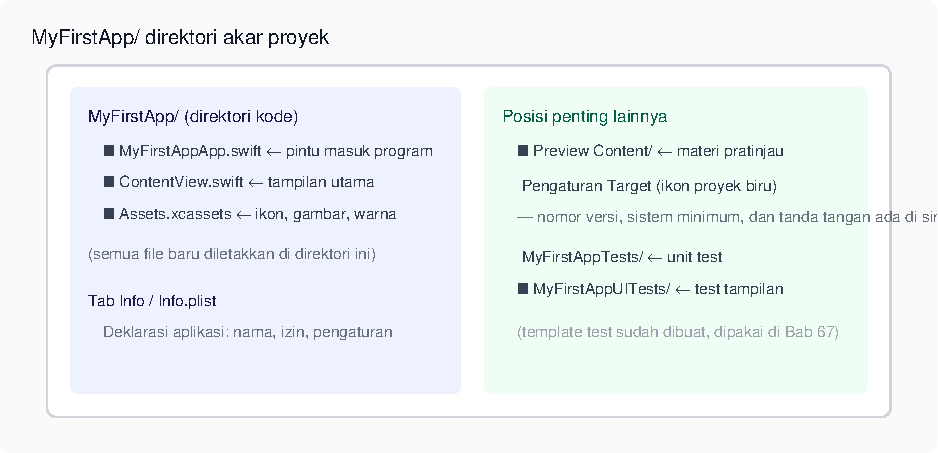
\includegraphics[width=0.92\linewidth]{figures/fig-di-liu-shi-zhang-1}
\\[2pt]\small Gambar 2: Struktur proyek Xcode yang wajib dipahami pemula
\end{center}

\begin{itemize}
  \item MyFirstAppApp.swift: pintu masuk program; di SwiftUI isinya hanya beberapa baris — "nyalakan, lalu tampilkan layar utama";
  \item ContentView.swift: tampilan layar utama; semua yang kamu lihat sekarang ada di sini;
  \item Assets.xcassets: gudang aset — ikon, gambar, dan warna ditaruh di sini;
  \item Pengaturan Target: tekan ikon proyek biru di kiri untuk masuk; nomor versi, versi iOS minimum, dan penandatanganan semuanya ada di dalamnya. Nama tampilan App dan ikon juga diatur di sini.
\end{itemize}

\booksection{Debug di perangkat asli: Memasang App ke iPhone-mu}

\booksection{Trik efisiensi Xcode: Lima “cheat shortcut” untuk pemula}

Kalau lima ini sudah terbiasa, kamu akan tampak “sangat profesional”:

\begin{center}
\begin{tabularx}{\linewidth}{|X|X|X|}
\hline
\textbf{Aksi} & \textbf{Shortcut} & \textbf{Fungsi} \tabularnewline
\hline
Jalankan & CmdR & Kompilasi dan langsung berjalan \tabularnewline
Membuka/mengalihkan pratinjau kanvas & OptionCmd & Sakelar pratinjau langsung (WYSIWYG) \tabularnewline
Merapikan indentasi & CtrlI & Merapikan otomatis indentasi kode yang dipilih \tabularnewline
Membuka file dengan cepat & CmdO & Ketik nama file, terbuka dalam sekejap (paling sering dipakai!) \tabularnewline
Memberi/menghapus komentar & Cmd/ & Mematikan/menyalakan kode sepintas saat debugging \tabularnewline
\hline
\end{tabularx}
\end{center}

\begin{center}\small\color{gray}Shortcut Xcode paling sering dipakai (paket lima pemula)\end{center}

Dua bonus tersembunyi lainnya: menjalankan beberapa Simulator sekaligus (iPhone dan iPad jalan bersamaan untuk membandingkan tata letak) dan pustaka potongan kode (tarik beberapa baris kode yang sering dipakai ke panel Snippets di kanan, nanti tinggal sisipkan sekali tekan) — pakai dulu alat efisiensinya, kecekatan tangan otomatis naik.

\booksection{Debug di perangkat asli: Memasang App ke iPhone-mu}

Simulator memang nyaman, tetapi perangkat asli adalah garis finisnya. Dengan Apple ID gratis pun bisa debug di perangkat asli:

\begin{enumerate}
  \item Sambungkan iPhone dengan kabel data (atau debug nirkabel lewat Wi-Fi yang sama);
  \item Pada daftar perangkat di bagian atas Xcode pilih ponselmu; pertama kali akan diminta masuk Apple ID dan penandatanganan dikonfigurasi otomatis;
  \item Di iPhone buka [Pengaturan] [Umum] [VPN \& Manajemen Perangkat] percayai sertifikat pengembangmu;
  \item Tekan >, dan App terpasang di perangkat asli.
\end{enumerate}

\begin{tcbwarn}{Perhatian: "Batasan tujuh hari" akun gratis}
App bertanda tangan Apple ID gratis akan kedaluwarsa setelah 7 hari (jalankan ulang sekali untuk memperpanjang). Ini mekanisme anti penyalahgunaan Apple dan untuk tahap belajar sepenuhnya cukup; akun pengembang berbayar (99 dolar AS/tahun) tak punya batasan ini — dibahas rinci di Bab 67.

\end{tcbwarn}

\booksection{Uji coba pertama + Pertolongan pertama error umum}

\booksection{Uji coba pertama + Pertolongan pertama error umum}

Buka ContentView.swift, ganti tulisan di dalam Text(“Hello, world!”) dengan namamu, tekan CmdR untuk menjalankan ulang — beberapa detik kemudian namamu tampil di Simulator. Selamat, kamu baru saja menuntaskan siklus lengkap pertamamu “ubah kode kompilasi pasang jalankan”.

\begin{center}
\begin{tabularx}{\linewidth}{|X|X|X|}
\hline
\textbf{Gejala error} & \textbf{Penyebab umum} & \textbf{Obatnya} \tabularnewline
\hline
Error Signing & Team belum dipilih, sertifikat kedaluwarsa & Di Target Signing centang akunmu; akun gratis tinggal jalankan ulang sekali \tabularnewline
Simulator layar hitam / tak mau terbuka & Image Simulator rusak & Menu Device Erase All Content; atau hapus lalu tambahkan ulang Simulator \tabularnewline
Unduhan Xcode lambat / gagal terpasang & Koneksi App Store tidak stabil & Ganti waktu; atau unduh paket offline .xip dari situs pengembang Apple \tabularnewline
\hline
\end{tabularx}
\end{center}

\begin{center}\small\color{gray}Tabel pertolongan pertama error lingkungan pemula\end{center}

\begin{tcbpractice}{Praktik: Tuntaskan daftar "ritual pengembangan"mu}
(1) Pasang Xcode dan jalankan Simulator sampai jalan; (2) jalankan App-mu sekali di perangkat asli dan simpan tangkapan layarnya sebagai kenangan; (3) ganti tulisan Hello dengan namamu; (4) ubah nama tampilan App menjadi “App Pertamaku” di pengaturan Target. Setelah empat langkah ini selesai, kamu resmi menjadi orang yang punya karya.

\end{tcbpractice}

\begin{tcbsummary}{Ringkasan bab}
\begin{itemize}
  \item Syarat mutlak: Mac + Xcode; tanpa Mac, belajar bahasanya dulu lewat Swift Playgrounds di iPad
  \item Xcode dipasang dari App Store; versi baru menuntut sistem baru, jangan tunda pembaruan
  \item Lima unsur proyek baru: nama, Team, pengenal organisasi, SwiftUI, Swift
  \item Jurus hafalan proyek: semua kode ada di folder MyFirstApp/; pengaturan Target mengurus versi dan penandatanganan
  \item Debug perangkat asli dengan Apple ID gratis punya batas tanda tangan 7 hari; akun berbayar tak ada batasan ini
  \item Rutinitas pengembangan = ubah kode CmdR lihat hasil, berulang terus
\end{itemize}

\end{tcbsummary}
